% ---------------------------------------------------------------- Task 2
\subsection{Task 2: our own hypotheses}

While exploring the data for Task 1 we noticed some patterns that the given
hypotheses did not cover: almost nobody stopped with a grade below 4, some
re-attempts took under a minute and got full marks, and two questions were often
left blank. We built our five hypotheses around these observations and around
ideas from the literature in Section~\ref{sec:background}. We also chose
hypotheses that need different kinds of charts, so that together they show
different parts of the data.

% ............................................................ H6
\subsubsection{H6 -- Do students re-attempt to pass, not to get full marks?}
\label{sec:h6}

\begin{hyp}{H6}
Students re-attempt a quiz mainly to reach a pass mark. Once they reach it,
most of them stop, even if they could still improve.
\end{hyp}

\textbf{How we tested it.} For every finished attempt we checked whether the
same student made another attempt on the same quiz. We then compared this
``try again'' rate across grades. If H6 is true, the rate should drop
sharply at one grade (the pass mark), not slowly as the grade goes up. We also
looked at where re-attempting students finally stopped.

\textbf{Why this chart.} Panel (a) uses grouped bars because we are comparing
a \emph{proportion} (which starts at zero) across ordered grades and three
quizzes; the shaded background marks grades below 4. Panel (b) uses 100\%
stacked bars with an ordered light-to-dark scale, which shows a
part-to-whole split of final grades and lets us compare two groups on the same
length scale. We did not use pie charts because two pies are hard to compare.

\begin{figure}[H]
\centering
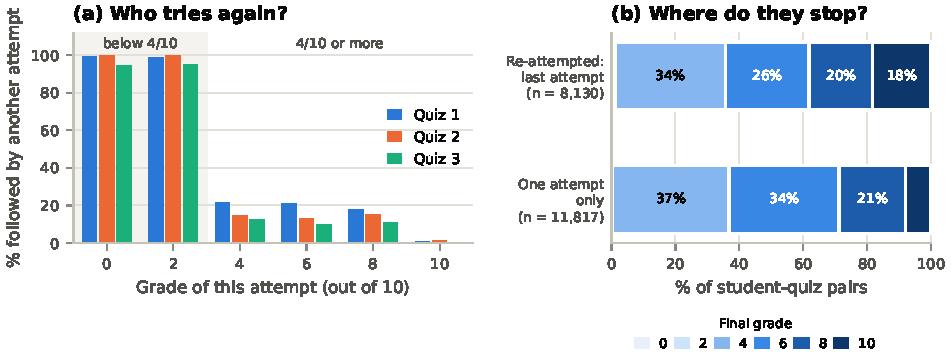
\includegraphics[width=\linewidth]{fig07_h6_pass_mark.pdf}
\caption{H6. (a) Share of attempts that were followed by another attempt on the
same quiz, by grade. (b) Final grade of students who re-attempted (their last
attempt) compared with students who made only one attempt.}
\label{fig:h6}
\end{figure}

\begin{mctable}
(a) re-attempt rate & Line (bar) & Length / vertical position $\rightarrow$ \% followed by another attempt; horizontal position $\rightarrow$ grade; hue $\rightarrow$ quiz \\
(a) fail zone & Area (background) & Grey shade $\rightarrow$ grades below 4 \\
(b) final grade split & Line (bar segment) & Length $\rightarrow$ share; lightness (ordered blue) $\rightarrow$ final grade \\
\end{mctable}

\textbf{What we see.} Panel (a) shows a cliff, not a slope. After a grade of 0
or 2, students tried again 98.7\% of the time. After a grade of 4, 6 or 8 the
rate falls to only 15.6\%, and after 10 it is 0.8\%. The drop happens exactly
between 2 and 4 in all three quizzes, and the rates for 4, 6 and 8 are almost
the same, so it is not simply ``the higher the grade, the less need to retry''.
The split is very strong (Cram\'er's $V$ = 0.78). Panel (b) shows where
students stop: 34.5\% of re-attempting students stopped at exactly 4/10, and
only 18\% went on to full marks. Among the 11,817 student--quiz pairs with only
one attempt, just 25 had a grade below 4. Together this strongly suggests that
the course uses 4/10 (40\%) as the pass mark, and that students treat it as the
goal. This is a clear example of satisficing \citep{simon1956rational}.

\begin{decision}
\textbf{Decision: \accepted.} Students below 4/10 almost always try again;
students at 4/10 or above almost always stop, and about a third of re-attempters
stop exactly at 4. Re-attempts are used to pass, not to master the material.
\end{decision}

% ............................................................ H7
\subsubsection{H7 -- Do instant re-attempts reuse the feedback?}
\label{sec:h7}

\begin{hyp}{H7}
When students are allowed to re-attempt immediately, the re-attempt gives a much
larger gain (they reuse the answers they have just seen in the feedback). When
there is a waiting time between attempts, this effect disappears.
\end{hyp}

\textbf{How we found it.} In H1 we saw re-attempts with full marks in about a
minute. To understand them we plotted the waiting time before every re-attempt
against the date. This showed something we did not expect: up to 12 May 2022
many re-attempts started within a minute of the previous one, but from 13 May
2022 \emph{no} re-attempt starts less than 120 minutes after the previous
attempt ended. The minimum waiting time after that date is exactly 120 minutes.
This looks like Moodle's ``enforced delay between attempts'' setting being
switched on with a value of 2 hours \citep{moodle_settings}. It gives us a
natural experiment: the same quizzes, before and after a waiting time was
added.

\textbf{Why this chart.} Panel (a) is a scatter plot because we want to see
every individual re-attempt and spot a sudden change; the y-axis is on a log
scale because waiting times go from seconds to months. We used colour for
\emph{emphasis}: re-attempts with 10/10 are orange and everything else is grey,
so the cluster of perfect, instant re-attempts stands out. Panel (b) uses 100\%
stacked bars to compare the grade distribution of three groups of re-attempts
on one length scale, with the sample size and the mean gain written above each
bar.

\begin{figure}[H]
\centering
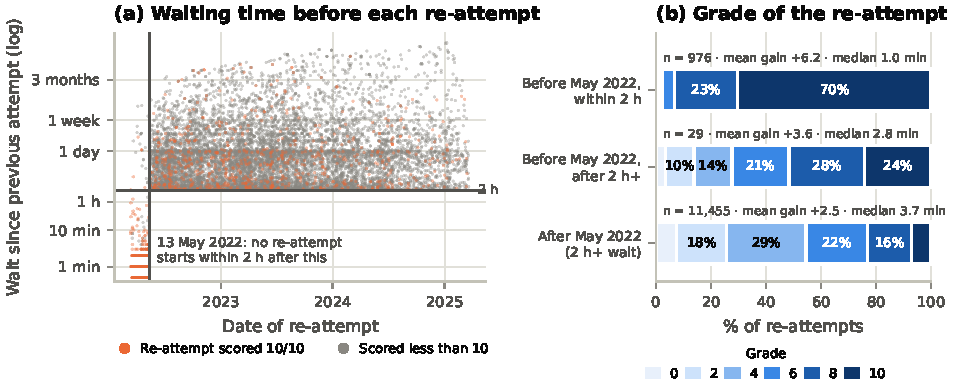
\includegraphics[width=\linewidth]{fig08_h7_retake_delay.pdf}
\caption{H7. (a) Waiting time before each of the 12,460 re-attempts, by date
(log scale). Orange = re-attempt scored 10/10. (b) Grade of the re-attempt for
three groups: before 13 May 2022 within 2 hours, before 13 May 2022 after 2+
hours, and after 13 May 2022 (always 2+ hours).}
\label{fig:h7}
\end{figure}

\begin{mctable}
(a) each re-attempt & Point & Horizontal position $\rightarrow$ date; vertical position (log) $\rightarrow$ waiting time; hue (orange vs.\ grey) $\rightarrow$ full marks or not \\
(a) reference & Line & Position $\rightarrow$ 2-hour floor and change date \\
(b) grade split & Line (bar segment) & Length $\rightarrow$ share of re-attempts; lightness (ordered blue) $\rightarrow$ grade; vertical position $\rightarrow$ group \\
\end{mctable}

\textbf{What we see.} Before the change, 976 of the 1,005 re-attempts started
within two hours, most of them within a minute. These quick re-attempts scored
9.2/10 on average, 70\% got full marks, and the median attempt took only 1.0
minute. The average gain over the previous attempt was +6.2 marks. After the
change, the average gain fell to +2.5 marks, only 7\% of re-attempts got full
marks, and the median time went up to 3.7 minutes. The difference in gains is
very large (Mann--Whitney $p < 0.001$; a random quick re-attempt gains more than
a random later one 84\% of the time). The earlier students were not stronger: their
previous grade was similar (3.0 vs.\ 2.4 on average), and their first-attempt
grades were in fact lower (3.7 vs.\ 4.5). A five-question
quiz cannot honestly be read and answered in one minute
\citep{wise2005response}, so the most likely explanation is that students were
copying the correct answers shown in the review of the previous attempt, a form
of ``gaming the system'' \citep{baker2004offtask, alexandron2017copying}.

The 29 re-attempts before May 2022 that did wait two hours or more gained +3.6
on average, between the two other groups. This group is small, so we do not
read much into it.

\begin{decision}
\textbf{Decision: \accepted.} Instant re-attempts gave very large, very fast
gains (+6.2 marks in about a minute, 70\% full marks). Once a two-hour wait was
enforced, these disappeared (+2.5 marks, 7\% full marks). This also explains
the fast, high-scoring re-attempts in H1 and H5.
\end{decision}

% ............................................................ H8
\subsubsection{H8 -- Does a good Quiz 1 result carry over to later quizzes?}
\label{sec:h8}

\begin{hyp}{H8}
Students who do well on Quiz 1 also do well on Quiz 2 and Quiz 3.
\end{hyp}

\textbf{How we tested it.} We used each student's \emph{first-attempt} grade on
each quiz (6,635 students who finished all three) and put it into three bands:
0--2 (failed), 4 (just passed) and 6--10 (good). We then followed each student
across the quizzes. We also computed Spearman's $\rho$ between the raw grades.

\textbf{Why this chart.} We want to see how groups of students \emph{move}
between bands over three steps. An alluvial diagram is made for this
\citep{rosvall2010mapping}: the blocks show how big each band is in each quiz,
and the ribbons show how many students move from one band to another. We
coloured every ribbon by the student's band in Quiz 1, so a reader can follow,
for example, the dark ``good in Quiz 1'' group all the way to Quiz 3. Panel (b)
then gives one clear number per Quiz 1 band using a bar chart with confidence
intervals, because the alluvial diagram is good for an overview but not for
reading exact values.

\begin{figure}[H]
\centering
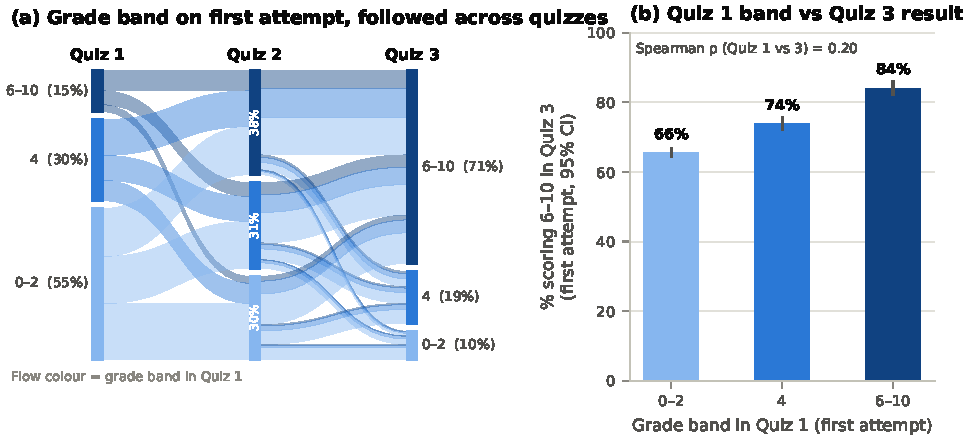
\includegraphics[width=\linewidth]{fig09_h8_carry_over.pdf}
\caption{H8. (a) Alluvial diagram of first-attempt grade bands across the three
quizzes; ribbon colour = band in Quiz 1. (b) Share of students who scored 6--10
on their first attempt in Quiz 3, by their band in Quiz 1.}
\label{fig:h8}
\end{figure}

\begin{mctable}
(a) band block & Area (rectangle) & Vertical length $\rightarrow$ share of students; horizontal position $\rightarrow$ quiz; vertical position $\rightarrow$ band (ordered); lightness $\rightarrow$ band \\
(a) ribbon & Area (flow) & Width $\rightarrow$ number of students moving; lightness $\rightarrow$ band in Quiz 1 \\
(b) outcome & Line (bar) + error bar & Length $\rightarrow$ \% scoring 6--10 in Quiz 3; lightness $\rightarrow$ Quiz 1 band \\
\end{mctable}

\textbf{What we see.} The direction is as expected: 84\% of students who scored
6--10 in Quiz 1 also scored 6--10 in Quiz 3, compared with 74\% of those who
scored 4 and 66\% of those who scored 0--2. But the alluvial diagram mostly
shows a lot of \emph{mixing}. Many students who failed Quiz 1 at first are in
the top band of Quiz 3, and only 43\% of the students in the top band of Quiz 1
stayed in the top band for both later quizzes. The correlation between
first-attempt grades is weak for every pair of quizzes ($\rho$ = 0.20 for
Quiz 1--2, 0.20 for 1--3 and 0.21 for 2--3; Cram\'er's $V$ = 0.11). One reason
is that the quizzes are very different in difficulty (Figure~\ref{fig:overview}c),
but even inside the same quiz the ranking of students changes a lot.

\begin{decision}
\textbf{Decision: \partly.} The direction is right (good in Quiz 1 $\rightarrow$
more likely to be good in Quiz 3), but the link is weak ($\rho \approx 0.2$).
A student's Quiz 1 result is a poor predictor of how they will do later, so
teachers should not label students early based on Quiz 1.
\end{decision}

% ............................................................ H9
\subsubsection{H9 -- Did later groups of students do better?}
\label{sec:h9}

\begin{hyp}{H9}
Students who took the quizzes later (2024--2025) score higher on their first
attempt than students who took them earlier (2022).
\end{hyp}

\textbf{How we tested it.} We grouped students into \emph{cohorts} by the
half-year of their first attempt on each quiz, and plotted the mean
first-attempt grade and the share of students who needed a re-attempt for
each cohort.

\textbf{Why this chart.} Cohorts are ordered in time, so a line chart is the
best fit; the lines are labelled directly at their ends, so no legend is
needed, and the 95\% confidence bands show which changes are bigger than the
noise. We put the grade and the re-attempt share in two separate panels instead
of one chart with two y-axes, because they are on different scales.

\begin{figure}[H]
\centering
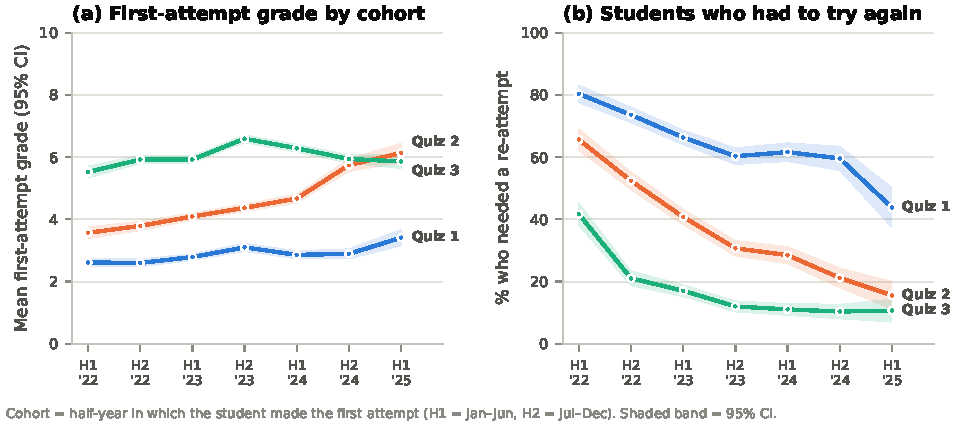
\includegraphics[width=\linewidth]{fig10_h9_cohort_trend.pdf}
\caption{H9. (a) Mean first-attempt grade by cohort (half-year). (b) Share of
students in each cohort who made more than one attempt.}
\label{fig:h9}
\end{figure}

\begin{mctable}
Cohort value & Point + line & Vertical position $\rightarrow$ mean grade or \% re-attempting; horizontal position $\rightarrow$ half-year (ordered); hue $\rightarrow$ quiz \\
Uncertainty & Area & Band height $\rightarrow$ 95\% CI \\
\end{mctable}

\textbf{What we see.} The three quizzes behave differently. Quiz 2 shows a big
and steady rise, from a mean of 3.6 in the first half of 2022 to 6.1 in early
2025 (\rhoeq{0.24}), with a jump in the second half of 2024. Quiz 1 rises only a
little, from 2.6 to 3.4 (\rhoeq{0.08}). Quiz 3 goes up until 2023 and then
comes back down (5.5, 6.6, then 5.9), so it has no clear trend. In panel (b)
the share of students who needed a re-attempt falls in all three quizzes (Quiz
1: 80\% to 44\%; Quiz 2: 66\% to 16\%; Quiz 3: 42\% to 11\%). Part of this fall
is caused by fewer students failing, and part by the two-hour delay from H7:
after it was introduced, far fewer students who had already passed tried again
just to improve.

We cannot say for sure \emph{why} Quiz 2 got easier. Figure~\ref{fig:h2}c shows
that Q2.1 and Q2.2 became much easier at the same time (from 45\% to 65\% and
from 46\% to 61\% between the two halves of 2024) while Q3.2 and Q3.3 became
harder. Changes this sudden look more like edits to the questions than a slow
change in students. Answers being shared between cohorts is another
possibility. Also, students in the last half-year had less time before the data
was exported, so their re-attempt share may be slightly too low.

\begin{decision}
\textbf{Decision: \partly.} Later cohorts did clearly better in Quiz 2, a
little better in Quiz 1, and not better in Quiz 3. Fewer students needed a
re-attempt in every quiz.
\end{decision}

% ............................................................ H10
\subsubsection{H10 -- Is a blank answer a sign of low effort?}
\label{sec:h10}

\begin{hyp}{H10}
Leaving a question blank is a sign of low effort: attempts with a blank answer
are finished faster and also score lower on the questions that were answered.
\end{hyp}

\textbf{How we tested it.} Only two questions are left blank often: Q1.4 (9.0\%
of first attempts) and Q2.5 (9.1\%). For these two, we compared first attempts
where the question was left blank with those where it was answered, on three
things: time taken, marks on the \emph{other four} questions (so the blank
itself does not count) and the share of attempts made by Low-tier students.

\textbf{Why this chart.} Time is skewed, so panel (a) uses box plots on a log
scale, which show the median and spread rather than a single average. Panels
(b) and (c) compare a mean and a proportion between two groups. The same layout
is used in all three panels, with hollow marks for ``answered'' and filled marks
for ``blank'', so the eye can move across the panels and read the same contrast
three times. Quiz colours stay the same as in all other figures.

\begin{figure}[H]
\centering
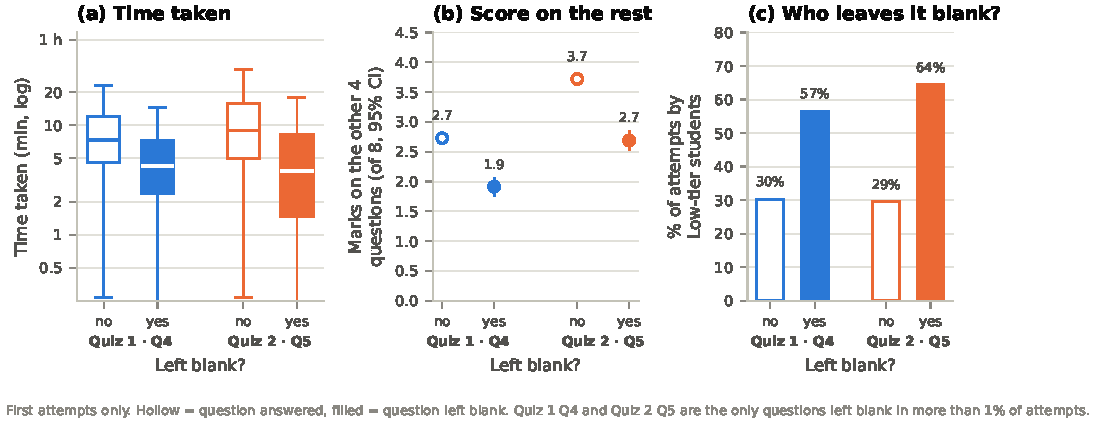
\includegraphics[width=\linewidth]{fig11_h10_blank_answers.pdf}
\caption{H10. First attempts for the two questions that are often left blank.
(a) Time taken. (b) Marks on the other four questions (out of 8) with 95\% CI.
(c) Share of these attempts made by Low-tier students.}
\label{fig:h10}
\end{figure}

\begin{mctable}
(a) time & Box plot (lines + area) & Vertical position (log) $\rightarrow$ median, quartiles and range of time \\
(b) other marks & Point + error bar & Vertical position $\rightarrow$ mean marks on other questions \\
(c) Low-tier share & Line (bar) & Length $\rightarrow$ \% Low-tier \\
All panels & -- & Fill (hollow vs.\ filled) $\rightarrow$ answered vs.\ blank; hue $\rightarrow$ quiz \\
\end{mctable}

\textbf{What we see.} All three panels tell the same story. Attempts that left
Q1.4 blank took a median of 4.3 minutes against 7.3 minutes for those that
answered it, and for Q2.5 it was 3.8 against 8.9 minutes. One in five (20\%) of
the Q1.4 blanks and 30\% of the Q2.5 blanks were finished in under two minutes,
compared with 6\% and 8\% of the others. These students also scored lower on
the questions they \emph{did} answer: 1.9 vs.\ 2.7 out of 8 in Quiz 1, and 2.7
vs.\ 3.7 in Quiz 2 (both $p < 0.001$). More than half of the blank attempts
came from Low-tier students (57\% and 64\%), against about 30\% of the answered
ones. The blank rate also falls steadily with tier: 15.5\% of Low, 7.4\% of
Medium and 2.5\% of High students left Q1.4 blank. This fits the idea of rapid,
low-effort responding described by \citet{wise2005response}.

\begin{decision}
\textbf{Decision: \accepted.} Attempts with a blank answer were about twice as
fast and scored lower on the other questions, and they came mostly from
low-performing students. A blank answer is a useful, cheap warning sign of low
effort.
\end{decision}
